\documentclass[14pt]{extarticle}
\usepackage{extsizes}
\usepackage{geometry}
\geometry{margin=0.5in}

%% for images
\usepackage{graphicx}
\graphicspath{ {images/} }

%% language support
\usepackage[T1,T2A]{fontenc}
\usepackage[utf8]{inputenc}
\usepackage[english,russian]{babel}

\usepackage{amsmath}
\usepackage{tikz}

%% hyperrefs
\usepackage{hyperref}
\hypersetup{
    colorlinks,
    citecolor=black,
    filecolor=black,
    linkcolor=black,
    urlcolor=black
}

\title{БДЗАААААААААААААААААААААААААААААА}
\author{Ну я}

\begin{document}
\maketitle
Это нужно знать всем детям! \\\\
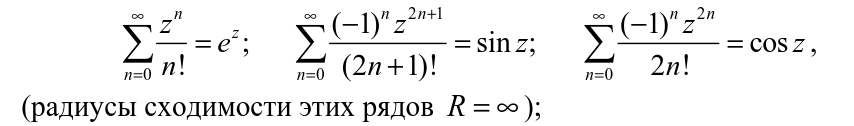
\includegraphics[width=450pt]{img1.png} \\
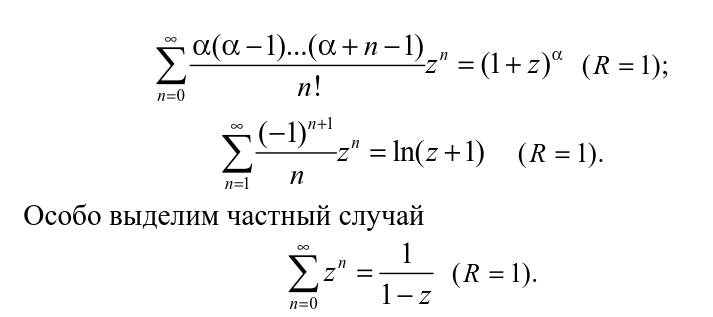
\includegraphics[width=350pt]{img2.png} \\
Удобное обозначение: \\
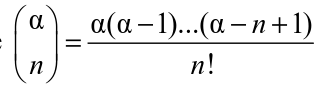
\includegraphics[width=150pt]{img3.png} \\

7. Заданную функцию $f(z)$ разложить в ряд Тейлора в точке $z_0$: 
$$f(z) = \frac{2z}{\sqrt{4-z^2}}, \ z_0 = 0$$
$$\frac{2z}{\sqrt{4-z^2}} = \frac{z}{\sqrt{1-\frac{z^2}{4}}}=
z \ * \ \left(1-\frac{z^2}{4}\right)^{-\frac{1}{2}}=
\sum_{n=0}^{\infty}\begin{pmatrix}
    -\frac{1}{2} \\
    n
\end{pmatrix}\frac{(-z^2)}{4^n}^n=$$
$$=
\sum_{n=0}^{\infty}\begin{pmatrix}
    -\frac{1}{2} \\
    n
\end{pmatrix}\frac{(-1)^n z^{2n}}{2^{2n}}$$

8. Заданную функцию $f(z)$ разложить в ряд Лорана в кольце
$a < |z-z_0| < b$ и в окрестности точки $z=\infty$:
$$f(z)=\frac{2z}{(z-1)(z^2+9)}, \ 1<|z|<3, \ z=\infty$$
$$f(z)=\frac{2z}{(z-1)(z^2+9)}=\frac{1}{5} \ \frac{1}{z-1}+
\left(-\frac{1}{5}z+\frac{9}{5}\right) \ \frac{1}{(z-3i)(z+3i)}
= f_1(z)+f_2(z)$$ \\
1) в кольце \\\\
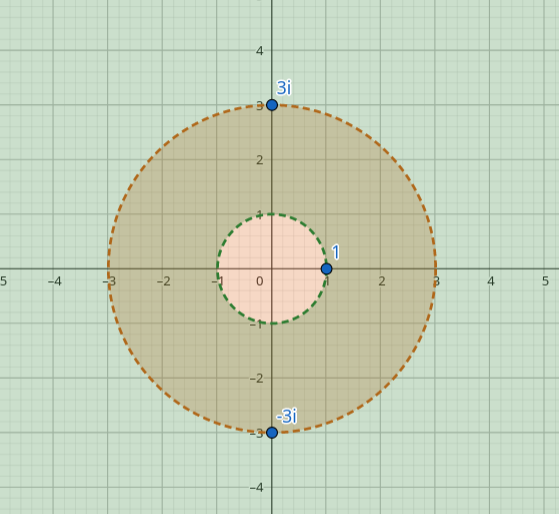
\includegraphics[width=300pt]{img4.png} \\
Точки $\pm 3i$ лежат вне кольца, потому 2е слагаемое соответствует
правильной части (раскладываем по степеням $z$); 
аналогично, точка $1$ лежит внутри кольца и 
1е слагаемое соответствует главной части (по степеням $\frac{1}{z}$). 

$$f_1(z) = \frac{1}{5} \ \frac{1}{z-1} = \frac{1}{5} \
\frac{1}{z} \ \frac{1}{1-\frac{1}{z}} = 
\frac{1}{5} \ \frac{1}{z} \sum_{n=0}^{\infty}\frac{1}{z^n} = 
\frac{1}{5} \sum_{n=0}^{\infty}\frac{1}{z^{n+1}} $$

$$f_2(z) = \left(-\frac{1}{5}z+\frac{9}{5}\right) \ \frac{1}{z^2+9}=
-\frac{1}{5} \ \frac{z-9}{z^2+9}=
-\frac{1}{5} 
\left(\frac{1-3i}{2} \ \frac{1}{z+3i} 
+ \frac{1+3i}{2} \ \frac{1}{z-3i}\right)=$$

$$= -\frac{1}{5} 
\left(\frac{1-3i}{6i} \ \frac{1}{1 + \frac{z}{3i}} 
- 
\frac{1+3i}{6i} \ \frac{1}{1 - \frac{z}{3i}}\right)=$$

$$= -\frac{1}{5} 
\left(\left(-\frac{1}{2}+\frac{1}{6}i\right) \ \frac{1}{1 + \frac{z}{3i}} 
+
\left(-\frac{1}{2}-\frac{1}{6}i\right) \ \frac{1}{1 - \frac{z}{3i}}\right)=$$

$$= -\frac{1}{5}
\left(\left(-\frac{1}{2}+\frac{1}{6}i\right)\sum_{n=0}^{\infty}(-1)^n
\frac{z^n}{(3i)^n}+\left(-\frac{1}{2}-\frac{1}{6}i\right)
\sum_{n=0}^{\infty}
\frac{z^n}{(3i)^n}\right)=$$

$$= -\frac{1}{10}\sum_{n=0}^{\infty}\frac{z^ni^n}{3^n}\left(
{\left(-1+\frac{1}{3}i\right)}
-(-1)^n\left(1+\frac{1}{3}i\right)\right)$$

Получим\\
$$f(z) = f_1(z) + f_2(z) 
= \frac{1}{5} \sum_{n=0}^{\infty}\frac{1}{z^{n+1}} +
\left(-\frac{1}{10}\right) \sum_{n=0}^{\infty}\frac{z^ni^n}{3^n}\left(
{\left(-1+\frac{1}{3}i\right)}
-(-1)^n\left(1+\frac{1}{3}i\right)\right)$$

2) в окрестности бесконечности \\
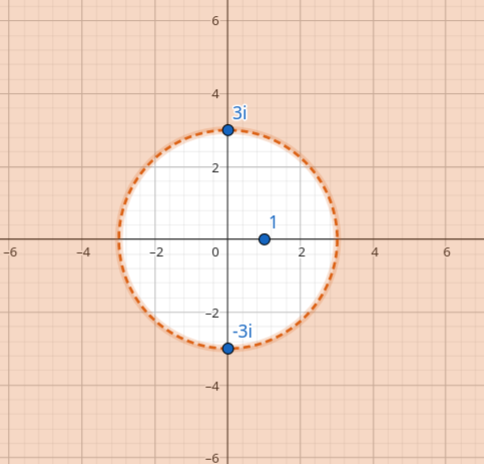
\includegraphics[width=300pt]{img5.png} \\
Раскладываем по степеням $\frac{1}{z}$. Для этого преобразуем $f_2(z):$
$$f_2(z) = -\frac{1}{5} 
\left(\frac{1-3i}{2} \ \frac{1}{z+3i} 
+ \frac{1+3i}{2} \ \frac{1}{z-3i}\right) = $$
$$= -\frac{1}{5} 
\left(\frac{1-3i}{2} \ \frac{1}{z} \ \frac{1}{1+\frac{3i}{z}} 
+ \frac{1+3i}{2} \ \frac{1}{z} \ \frac{1}{1-\frac{3i}{z}}\right) = $$

$$= -\frac{1}{10} 
\left((1-3i) \ \frac{1}{z} \ \frac{1}{1+\frac{3i}{z}} 
+ (1+3i) \ \frac{1}{z} \ \frac{1}{1-\frac{3i}{z}}\right) = $$

$$= -\frac{1}{10} 
\left((1-3i)\sum_{n=0}^{\infty}(-1)^n\frac{3^n i^n}{z^{n+1}}
+ (1+3i)\sum_{n=0}^{\infty}\frac{3^n i^n}{z^{n+1}}\right)=$$

$$= -\frac{1}{10} 
\left(\sum_{n=0}^{\infty}\frac{3^n i^n}{z^{n+1}}
((-1)^n(1-3i)+(1+3i))\right)$$

Итого\\
$$f(z)= f_1(z) + f_2(z) = 
\frac{1}{5} \sum_{n=0}^{\infty}\frac{1}{z^{n+1}} + 
\left(-\frac{1}{10}\right) 
\left(\sum_{n=0}^{\infty}\frac{3^n i^n}{z^{n+1}}
((-1)^n(1-3i)+(1+3i))\right)=$$
$$=\left(-\frac{1}{10}\right)\sum_{n=0}^{\infty}
\frac{1}{z^{n+1}}\left(-2+3^n i^n((-1)^n(1-3i)+(1+3i))\right)$$
\\\\
9. Найти все особые точки аналитической функции, выяснить их
характер и исследовать поведение функции на бесконечности:
$$f(z)=\frac{1}{z-1+e^{-z}}+\cos{\frac{1}{z-1}}$$
Важно знать:\\
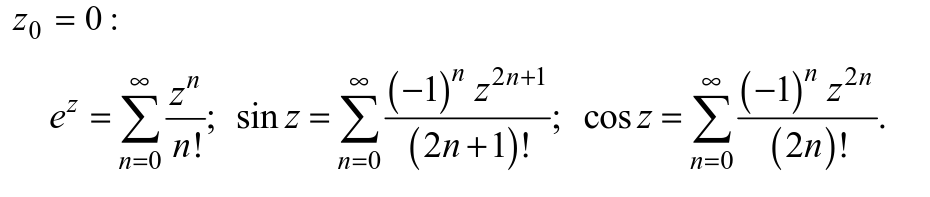
\includegraphics[width=400pt]{img7.png} \\
Изолированные особые точки: 
$$z-1=0 => z=1$$
$$z-1+e^{-z}=0 <=> 1-z = e^{-z} => z=0$$
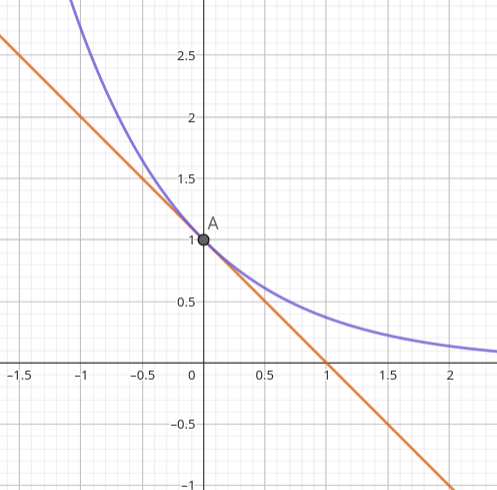
\includegraphics[width=200pt]{img6.png} \\
(если на бумаге, то вручную то же самое чертить - по графику видно,
что там ровно одна точка)
$$z\to 1: \ f(z) = \frac{1}{z-1 + \left(\frac{1}{e}\right)e^{1-z}}
+ \cos{\frac{1}{1-z}} = $$

$$=\frac{1}{-(1-z) + \left(\frac{1}{e}\right)\sum_{n=0}^{\infty}
\frac{(1-z)^n}{n!}}
+ \sum_{n=0}^{\infty}(-1)^n\frac{(\frac{1}{1-z})^{2n}}{(2n)!}$$
Главная часть содержит бесконечно много членов, поэтому $z=1$ -
\textcolor{red}{существенно особая точка}.
$$z\to 0: \lim_{z\to 0}f(z) = \lim_{z\to 0} \left(
\frac{1}{z-1+e^{-z}}+\cos{\frac{1}{z-1}}\right)=\infty$$
Таким образом, $z=0$ - полюс. Найдём порядок полюса. 
Для этого заметим, что $\cos{\frac{1}{z-1}}$ при $z\to 0$ стремится
тупо к константе, поэтому можем оставить для рассмотрения только 
$f_1(z) = \frac{1}{z-1+e^{-z}}$. Для поиска полюса рассмотрим обратную 
к ней, воспользуясь вот такой вот теормемой: \\
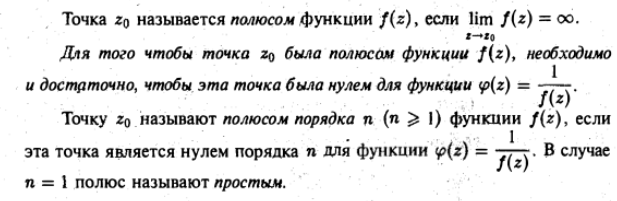
\includegraphics[width=500pt]{img8.png} \\
Кароче, 
$$\phi(z) = z-1+e^{-z}, \ \phi(z=0) = 0 - 1 + 1 = 0$$
$$\phi^{'}(z) = 1-e^{-z}, \ \phi^{'}(z=0) = 1 - 1= 0$$
$$\phi^{''}(z) = e^{-z}, \ \phi^{''}(z=0) = 1 \neq 0$$
Таким образом, $z=0$ - \textcolor{red}{полюс 2го порядка}.\\\\
Теперь $z=\infty$.
$$z\to \infty: \lim_{z\to \infty}f(z) = \lim_{z\to \infty} \left(
\frac{1}{z-1+e^{-z}}+\cos{\frac{1}{z-1}}\right)=
\lim_{z\to \infty} \left(
\frac{1}{z-1+0}+\cos{\frac{1}{z-1}}\right)=$$
$$= 0 + \cos 0 = 1$$
Т.е. бесконечность - \textcolor{red}{устранимая особая точка}.\\\\
10. Найти вычеты относительно всех изолированных особых точек
(включая $z=\infty$) функции:
$$f(z)=\frac{\sin2z}{e^{iz}-1}+z^2e^{\frac{1}{z}}$$
Итак, $z=0$.
$$\lim_{z\to 0} f(z) = \lim_{z\to 0} 
\left(\frac{\sin2z}{e^{iz}-1}+z^2e^{\frac{1}{z}}\right)=
\lim_{z\to 0} 
\left(\frac{2z}{e^{iz}-1}+\frac{e^{\frac{1}{z}}}{z^{-2}}\right)=
<\frac{0}{0}+\frac{\infty}{\infty}>=$$
$$=\lim_{z\to 0}\left(\frac{2}{ie^{iz}}
+\frac{-\frac{1}{z^2}e^{\frac{1}{z}}}{-\frac{2}{z^3}}\right)=
\frac{2}{i}+
\frac{1}{2}\lim_{z\to 0}\frac{e^{\frac{1}{z}}}{\frac{1}{z}}
=<\frac{2}{i} + \frac{1}{2}\frac{\infty}{\infty}>=
\frac{2}{i}+
\lim_{z\to 0}\frac{-\frac{1}{z^2}e^{\frac{1}{z}}}{-\frac{1}{z^2}}=\infty$$
Получился полюс. Очень жаль. Теперь придётся искать коэффициент перед
первым главным членом, так как это и есть вычет по определению.
К счастью, для этого есть формула, так что нам просто нужно 
найти порядок полюса. 
\end{document}
